\documentclass{article}

% if you need to pass options to natbib, use, e.g.:
%     \PassOptionsToPackage{numbers, compress}{natbib}
% before loading neurips_2020

% ready for submission
% \usepackage{neurips_2020}

% to compile a preprint version, e.g., for submission to arXiv, add add the
% [preprint] option:
%     \usepackage[preprint]{neurips_2020}

% to compile a camera-ready version, add the [final] option, e.g.:
%     \usepackage[final]{neurips_2020}

% to avoid loading the natbib package, add option nonatbib:
\usepackage{neurips2020}
\usepackage{amsmath}
\usepackage{graphicx}
\usepackage[utf8]{inputenc} % allow utf-8 input
\usepackage[T1]{fontenc}    % use 8-bit T1 fonts
\usepackage{hyperref}       % hyperlinks
\usepackage{url}            % simple URL typesetting
\usepackage{booktabs}       % professional-quality tables
\usepackage{amsfonts}       % blackboard math symbols
\usepackage{nicefrac}       % compact symbols for 1/2, etc.
\usepackage{microtype}      % microtypography
\usepackage{bm}
\usepackage{xr}
\externaldocument{suppcausalMARL}

\newcommand{\Mean}{{\mathbb{E}}}
\newcommand{\Var}{{\mbox{Var}}}
\newcommand{\Cov}{{\mbox{cov}}}
\newcommand{\Corr}{{\mbox{corr}}}
\newcommand{\diag}{{\mbox{diag}}}
\newcommand{\prob}{{\mathbb{P}}}
\newcommand\independent{\protect\mathpalette{\protect\independenT}{\perp}}
\newtheorem{lemma}{Lemma}
\newtheorem{thm}{Theorem}
\def\independenT#1#2{\mathrel{\rlap{$#1#2$}\mkern2mu{#1#2}}}
\DeclareMathOperator*{\argmin}{arg\,min}
\title{Spatiotemporal Causal Effects Evaluation:\\ A Multi-Agent Reinforcement Learning Framework}

% The \author macro works with any number of authors. There are two commands
% used to separate the names and addresses of multiple authors: \And and \AND.
%
% Using \And between authors leaves it to LaTeX to determine where to break the
% lines. Using \AND forces a line break at that point. So, if LaTeX puts 3 of 4
% authors names on the first line, and the last on the second line, try using
% \AND instead of \And before the third author name.

\author{%
	David S.~Hippocampus\thanks{Use footnote for providing further information
		about author (webpage, alternative address)---\emph{not} for acknowledging
		funding agencies.} \\
	Department of Computer Science\\
	Cranberry-Lemon University\\
	Pittsburgh, PA 15213 \\
	\texttt{hippo@cs.cranberry-lemon.edu} \\
	% examples of more authors
	% \And
	% Coauthor \\
	% Affiliation \\
	% Address \\
	% \texttt{email} \\
	% \AND
	% Coauthor \\
	% Affiliation \\
	% Address \\
	% \texttt{email} \\
	% \And
	% Coauthor \\
	% Affiliation \\
	% Address \\
	% \texttt{email} \\
	% \And
	% Coauthor \\
	% Affiliation \\
	% Address \\
	% \texttt{email} \\
}

\begin{document}
	
\maketitle

\begin{abstract}
	Online experiment is a default option for technological companies to make data-driven product decisions. Major challenge arise in experiments where multiple units in different areas receive sequences of treatments over time. Causal effects evaluation is extremely challenging in those experiments because (i) spatial and temporal proximities induce interference between locations and times; (ii) the large number of locations results in the curse of dimensionality; (iii) the short duration of the experiment leads to data scarcity. In this paper, we introduce a multi-agent reinforcement learning framework for carrying spatiotemporal causal effects evaluation and propose novel estimators for mean outcomes under different products that are consistent despite the high-dimensionality of state-action space. The proposed estimator works favourably in simulation experiments. We further illustrate our method using data from a ridesharing company to evaluate the effects of applying subsidizing policies in different areas. 
\end{abstract}
	
\section{Introduction}
Online experiment is a standard business strategy for technological companies to make data-driven product decisions. The existing literature on causal inference has mostly focused on the setting where no interference occurs, i.e., the outcome of each experimental unit depends only on its treatment status. This assumption is referred to as the stable unit treatment value assumption \citep[SUTVA,][]{rubin1980randomization,rubin1986comment} under a potential outcome framework \citep[see, e.g.,][]{rubin2005}. 

In many experiments, however, there are multiple units in different areas that receive sequences of treatments over time. For instance, suppose a ride-sharing company would like to evaluate the effect of applying different subsidizing policies to drivers in different spatial units of a city. Implementing a subsidizing policy at one location will attract drivers from other areas to that location, thus affecting the spatial distribution of drivers in the city. Consequently, the subsidizing policy at one location will impact outcomes of other areas, inducing interference between spatial units. In addition, the subsidizing policy at a given time will affect both current and future rewards, inducing interference over time. This leads to the violation of SUTVA.

\textbf{Contribution.} The focus of this paper is to evaluate the impact of multiple products in the presence of spatiotemporal interference, using data from online experiment. %Due to the budget constraint, each experiment lasts for only a few weeks. There are three major challenges here: (i) the presence of spatiotemporal interference; (ii) the curse of dimensionality resulting from the large number of locations; (iii) the data scarcity resulting from the short duration of the experiment. 
%leading to violation of 
Our contributions are multi-fold. First, we introduce a multi-agent reinforcement learning \citep[MARL, see e.g.,][]{nowe2012game} framework for spatiotemporal causal effects evaluation. Each spatial unit in the city is considered as an agent. In addition to the treatment-outcome pairs, it is assumed that each agent is associated with a set of time-varying confounding variables. This naturally leads to a multi-agent system. Under this framework, the carryover effects in space is modeled by the interactions between different agents. The carryover effects in time is modeled by the dynamic system transitions. See the causal diagram depicted in Figure \ref{fig1} for an illustration. Estimation of the mean outcome under different products is reduced to the off-policy evaluation problem in MARL. This addresses the challenge on spatiotemporal interference. 

Second, we propose a doubly-robust off-policy evaluation procedure in MARL. The proposed estimator requires estimation of the density ratio of the stationary state distribution and the Q-function associated with each single agent. The key ingredient of our method lies in learning the density ratio and Q-function based on mean-field approximation (see Section \ref{sec:method} for details) and aggregating these estimators properly to satisfy the doubly-robustness property. The mean field approximation effectively reduces the high-dimensional state-action space to a moderate scale, leading to a value estimator with decreased variance. The doubly-robustness guarantees our estimated value is consistent when either the density ratio or the Q-function is well-approximated, reducing its bias resulting from the mean-field approximation. This addresses the challenges on the curse of dimensionality. 

Third, we rigorously investigate the statistical properties of our estimator. %We establish its rate of convergence and derive its limiting distribution. %Consistency of our estimator requires the number of decision points $T$ to grow to infinity. 
In particular, we establish its doubly-robustness property (see Theorem \ref{thm:double}) and derive its ``oracle" property when both the density ratio and the Q-function are well approximated (see Theorem \ref{thm:oracleest}). The number of spatial units $N$ is allowed to be either bounded or diverge to infinity. As such, the proposed estimator offers a useful policy evaluation tool to a wide range of applications in the presence of spatiotemporal interference. 

%Finally, we introduce a potential outcome framework for 
%\subsection{Contributions}
\begin{figure}[!t]
	\centering
	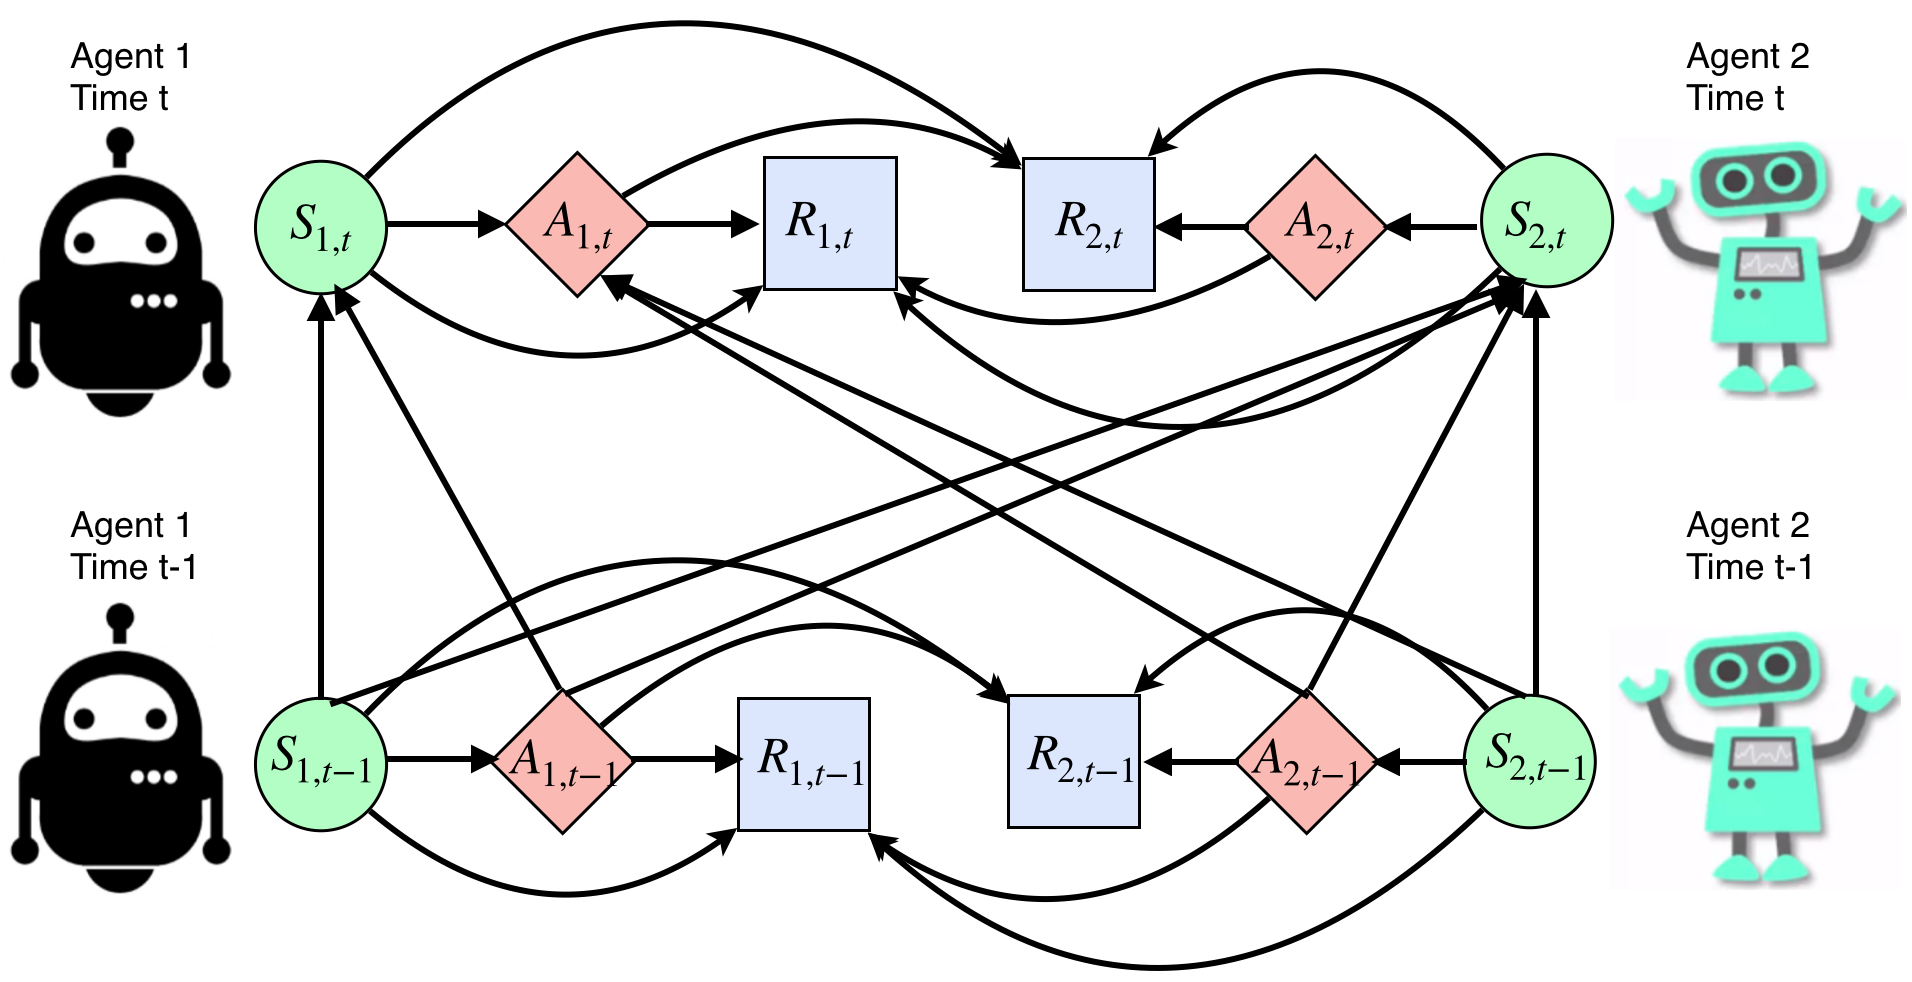
\includegraphics[width=9cm]{CausalDiagram.png}
	\vspace{-0.3cm}
	\caption{\small Causal diagram for a multi-agent system with two agents. $(S_{j,t},A_{j,t},R_{j,t})$ represents the state-treatment-outcome triplet of the $j$-th agent at time $t$.}\label{fig1}
\end{figure}

%\section{Related work}
\textbf{Related work.} There is a huge literature on causal inference. As commented before, most works considered settings without interference. Our work is related to research on space- or time-dependent casual effects evaluation \citep[see e.g.,][]{Hudgens2008,Eric2012,toulis2013estimation,dempsey2017stratified,Athey2018,Murphy2018,bhattacharya2019causal,Bojinov2019,ning2019Bayes}. However, none of the above cited works studied the interference effects in both space and time. In addition, the reinforcement learning framework has not been utilized in these papers to characterize the casual effects. 

In addition to the literature on causal inference, our work is also related to a line of research on MARL in the cooperative setting \citep[see e.g.,][for an overview]{zhang2019multi} and online control of infectious diseases \citep[see e.g.,][]{Laber2018}. Most works in the literature considered the \textit{policy optimization} problem where the objective is that agents collaborate to optimize a long-term reward. In particular, \cite{yang2018mean} developed a mean field Q-learning algorithms in the discounted-reward setting. %, and studied the convergence of the solution to Nash equilibrium. 
We remark that {\textit{policy evaluation}} is an ultimately different problem as policy optimization. On the other hand, the proposed value estimator relies on an estimated Q-function. To this end, we extend \cite{yang2018mean}'s proposal to the average-reward setting, which is more suitable for our application. In addition, we propose a mean field algorithm to approximate the density ratio of the stationary state distribution in a multi-agent system, in order to construct our doubly-robust estimates.

Furthermore, our work is also related to the literature on off-policy evaluation in reinforcement learning, in particular, on importance-sampling based or doubly-robust estimation of the value \citep[see e.g.,][]{thomas2015,jiang2016,liu2018,kallus2019efficiently,uehara2019minimax,tang2019doubly}. However, all the above cited papers considered a single-agent system, which is ultimately different from our setup.\vspace{-0.3cm}
%. To the best of our knowledge, mean field approximation of the density ratio has not been proposed in the existing literature. 

\section{Causality and MARL}\label{sec:causalMARL}\vspace{-0.2cm}
%\subsection{A causal framework for MARL}
In this section, we extend Robin's potential outcome framework to the multi-agent system. We assume there are only two treatments (actions) associated with the $i$-th spatial unit (agent), i.e. the action space $\mathcal{A}_i=\{0,1\}$. In our ride-sharing applications, the two treatments correspond to applying the subsidizing policy to a given area or not. For $1\le i\le N$, let $\mathbb{S}_i$ denote the state space associated with the $i$-th agent. In addition, let $\mathbb{S}_0$ denote the space of some global state variables in the system (such as time of day in our applications). The joint state and action spaces are given by $\mathbb{S}=\mathbb{S}_0 \times \mathbb{S}_1 \times \mathbb{S}_2 \times \cdots \times \mathbb{S}_N$ and $\mathcal{A}=\mathcal{A}_1\times \mathcal{A}_2 \times  \cdots \times \mathcal{A}_N=\{0,1\}^N$, respectively. 

For a sequence of $N$-dimensional vectors $\bm{a}_0,\bm{a}_1,\cdots, \bm{a}_t\in \{0,1\}^{N}$, define a treatment history vector $\bar{\bm{a}}_t=(\bm{a}_0^\top,\bm{a}_1^\top,\cdots,\bm{a}_t^\top)^\top$ up to time $t$. For each $i\in \{1,\cdots,N\}$, let $S_{i,t}^*(\bar{\bm{a}}_{t-1}) \in \mathcal{S}_i$ and $R_{i,t}^*(\bar{\bm{a}}_t)\in \mathbb{R}$ be the potential state and reward (outcome) associated with the $i$-th agent at time $t$, that would occur had all agents followed $\bar{\bm{a}}_t$. Similarly, let $S_{0,t}^*(\bar{\bm{a}}_{t-1})$ be the potential global state that would occur at time $t$ had all agents followed $\bar{\bm{a}}_{t-1}$. Note that different action histories would lead to different potential outcomes. More importantly, these potential outcomes cannot be directly observed. We only have access to those following actions selected by the agents (see Condition (CA) below). Consequently, causal inference is inherently a missing data problem. More specifically, let $\{(S_{0,t}, S_{i,t},A_{i,t},R_{i,t}):1\le i\le N,0\le t< T\}\cup \{S_{i,T}:0\le i\le N\}$ be the observed data where $S_{0,t}$ denotes the observed global state at time $t$, $(S_{i,t},A_{i,t},R_{i,t})$ stands for the observed state-action-reward triplet associated with the $i$-th agent at time $t$ and $T$ is the termination time of the experiment. 
Let $\bm{A}_t=(A_{1,t},\cdots,A_{N,t})^\top$ be the observed treatments at time $t$ and $\bar{\bm{A}}_t=(\bm{A}_0^\top,\bm{A}_1^\top,\cdots,\bm{A}_t^\top)^\top$. We make the following consistency assumption (CA).

(CA) $S_{i,t}=S_{i,t}^*(\bar{\bm{A}}_{t-1})$, $R_{i,t}=R_{i,t}^*(\bar{\bm{A}}_t)$ almost surely for any $i$ and $t$.

SUTVA requires $S_{i,t+1}^*$ and $R_{i,t}^*$ to be functions of $A_{i,t}$ only. The above condition extends SUTVA to settings with spatiotemporal interference. Specifically, these potential outcomes are allowed to depend on not only past treatments, but actions selected by other agents as well. 

The following sequential randomization assumption (SRA) guarantees our causal estimands are identifiable from the observed data. 

(SRA) $\bm{A}_t \independent \bm{W}^* |\{(S_{0,j},S_{i,j},A_{i,j},R_{i,j}): 1\le i\le N, 0\le j<t \}\cup \{S_{i,t}:0\le i\le N\}$ for any $t$ where $\bm{W}^*=\cup_{t\ge 0,\bar{\bm{a}}_t\in \{0,1\}^{N(t+1)} } \bm{W}_t^*(\bar{\bm{a}}_t)$ where $\bm{W}_t^*(\bar{\bm{a}}_t)$ denotes the set of potential outcomes following $\bar{\bm{a}}_t$ up to time $t$, i.e.,
\vspace*{-0.1cm}
\begin{eqnarray*}
	\bm{W}_t^*(\bar{\bm{a}}_t)=\{ (S_{0,j}^*(\bar{\bm{a}}_{j-1}), S_{i,j}^*(\bar{\bm{a}}_{j-1}), R_{i,j}^*(\bar{\bm{a}}_j)):1\le i\le N, 0\le j\le t \}.
\end{eqnarray*}

\vspace*{-0.2cm}
SRA is satisfied in our applications where $A_{i,t}$'s are i.i.d. Bernoulli random variables, independent of other observations. More generally, it automatically holds in randomized experiments where the distribution of $\bm{A}_t$ is completely determined by the observed state-action-reward history. However, this condition cannot be verified from data from observational studies. We note that CA and SRA are commonly imposed in sequential decision making problems \citep[see e.g.,][]{Murphy2003,robins2004,Zhang2013,ertefaie2014,Laber2018,luckett2019}. 

Let $\bm{S}_t^*(\bar{\bm{a}}_{t-1})=\{S_{0,t}^*(\bar{\bm{a}}_{t-1}), S_{1,t}^*(\bar{\bm{a}}_{t-1}),\cdots,S_{N,t}^*(\bar{\bm{a}}_{t-1})\}^\top$ be the potential state vector at time $t$. Next we introduce the Markov assumption (MA) and the conditional mean independence assumption (CMIA). These conditions assume the system dynamics are homogeneous over time, enabling consistent estimation of our causal estimands. 

(MA) There exists a Markov transition kernel $\mathcal{P}: \mathbb{S}\times \mathcal{A} \times \mathbb{S}\to \mathbb{R}$ such that for any $t \ge 0$, $\bar{\bm{a}}_t\in \{0,1\}^{N(t+1)}$ and $\mathcal{S}\in \mathbb{S}$, we have
\vspace*{-0.1cm}
\begin{eqnarray*}
	\prob \{\bm{S}_t^*(\bar{\bm{a}}_{t-1})\in \mathcal{S}|\bm{W}_{t-1}^*(\bar{\bm{a}}_{t-1})\}=\mathcal{P}(\mathcal{S};\bm{a}_{t-1},\bm{S}_{t-1}^*(\bar{\bm{a}}_{t-2})).
\end{eqnarray*}
\vspace*{-0.1cm}
(CMIA) There exist functions $r_1,\cdots,r_N$ such that for any $1\le i\le N$, $t\ge 0$, $\bar{\bm{a}}_t\in \{0,1\}^{N(t+1)}$,%, we have
%\vspace*{-0.1cm}
\begin{eqnarray*}
	\Mean \{R_{i,t}^*(\bar{\bm{a}}_{t})| \bm{S}_t^*(\bar{\bm{a}}_{t-1}),\bm{W}_{t-1}^*(\bar{\bm{a}}_{t-1})\}=r_i(\bm{a}_t,\bm{S}_t^*(\bar{\bm{a}}_{t-1})).
\end{eqnarray*}
Throughout this paper, we assume CA, SRA, MA and CMIA hold. 

%\subsection{Causal estimands in multi-agent systems}
We next describe our causal estimands. We focus on the class of non-dynamic policies indexed by an $N$-dimensional vector $\bm{\pi}=(\pi_1,\cdots,\pi_N)^\top \in \{0,1\}^N$. Under $\bm{\pi}$, the $i$-th spatial unit will receive the same treatment $\pi_i$ over time. We are interested in evaluating the average reward under $\bm{\pi}$. In our applications, this helps the company to decide whether to apply subsidizing policies to specific areas in a given city according to $\bm{\pi}$ or not, under some budget constraints. To this end, 
%we define the long-term value under $\bm{\pi}$ as
%\begin{eqnarray}\label{eqn:value}
%	V(\bm{\pi})=\lim_{t\to \infty} \frac{1}{N t}\sum_{i=1}^N \sum_{j=0}^t \Mean R_{i,t}^*(\bm{\pi})=\lim_{t\to \infty} \frac{1}{N t}\sum_{i=1}^N \sum_{j=0}^t \Mean r_{i}^*(\bm{\pi},\bm{S}^*_t(\bm{\pi})),
%\end{eqnarray}
%under CMIA, 
%where $\bm{S}^*_t(\bm{\pi})$ and $R_{i,t}^*(\bm{\pi})$ denote the potential outcomes that would occur at time $t$ had all agents followed the non-dynamic policy $\bm{\pi}$. The limit in \eqref{eqn:value} is well-defined provided that $r_i^*(\bm{\pi},\bm{s})$ is continuous in $\bm{s}$ and the stationary distribution of the Markov chain generated by the transition kernel $\mathcal{P}(\cdot;\bm{\pi},\cdot)$ is unique \citep[see e.g., Proposition 1 of][for details]{Breiman1960}. We next 
we present the average treatment effect (ATE) for multi-agent systems in the following definition. 

\textbf{Definition (ATE).} Given a control policy $\bm{\pi}_0$ and a new policy $\bm{\pi}_1$, ATE is defined as the difference between their long term values, 
\vspace{-0.2cm}
\begin{eqnarray}\label{eqn:ATE}
%\begin{split}
\hbox{ATE}(\bm{\pi}_0,\bm{\pi}_1)=\lim_{t\to \infty} \frac{1}{N t}\sum_{i=1}^N \sum_{j=0}^t \Mean R_{i,j}^*(\bm{\pi}_1)-\lim_{t\to \infty} \frac{1}{N t}\sum_{i=1}^N \sum_{j=0}^t \Mean R_{i,j}^*(\bm{\pi}_0),%\\
%=\lim_{t\to \infty} \frac{1}{N t}\sum_{i=1}^N \sum_{j=0}^t \Mean r_{i}^*(\bm{\pi}_1,\bm{S}^*_t(\bm{\pi}_1))-\lim_{t\to \infty} \frac{1}{N t}\sum_{i=1}^N \sum_{j=0}^t \Mean r_{i}^*(\bm{\pi}_0,\bm{S}^*_t(\bm{\pi}_0)),
%\end{split}		
\end{eqnarray}
where $\bm{S}^*_t(\bm{\pi})$ and $R_{i,t}^*(\bm{\pi})$ denote the potential outcomes that would occur at time $t$ had all agents followed the non-dynamic policy $\bm{\pi}$. %The second equality follows from CMIA. 
%The limits in \eqref{eqn:ATE} are well-defined provided that $r_i^*(\bm{\pi}_j,\bm{s})$ is continuous in $\bm{s}$ for $j\in \{0,1\}$, $i\in \{1,\cdots,N\}$, and that the stationary distribution of the Markov chain generated by the transition kernel $\mathcal{P}(\cdot;\bm{\pi}_j,\cdot)$ is unique for $j\in\{0,1\}$ \citep[see e.g., Proposition 1 of][for details]{Breiman1960}.

We focus on comparing a standard policy $\bm{\pi}_0$ with several new alternatives $\{\bm{\pi}_1,\bm{\pi}_2,\cdots,\bm{\pi}_m\}$. This requires to evaluate $\hbox{ATE}(\bm{\pi}_0,\bm{\pi}_\ell)$ for $\ell=1,2,\cdots,m$. By definition, it is equivalent to evaluate the value under each $\bm{\pi}_{\ell}$, i.e.,  $V(\bm{\pi}_{\ell})=\lim_{t\to \infty} (Nt)^{-1}\sum_{i=1}^N \sum_{j=0}^t \Mean R_{i,j}^*(\bm{\pi}_{\ell})$. Note that $V(\bm{\pi}_{\ell})$ can be represented by $N^{-1} \sum_{i=1}^N V_i(\bm{\pi}_{\ell})$ where $V_i(\bm{\pi}_{\ell})=\lim_{t\to \infty} t^{-1}\sum_{j=0}^t \Mean R_{i,j}^*(\bm{\pi}_{\ell})$. It suffices to estimate $V_i(\bm{\pi}_{\ell})$ for $i\in \{1,2,\cdots,N\}$. We detail our procedure in the next section. 
%We next introduce the notion of the Q-function under the potential outcome framework. 

%Consider a standard policy $\bm{\pi}_0$ and 

%When $r_i^*(\bm{\pi},\bm{s})$ is continuous in $\bm{s}$ and the stationary distribution of the Markov chain generated by the transition kernel $\mathcal{P}(\cdot;\bm{\pi},\cdot)$ is unique, it follows from Proposition 1 of 
\vspace{-0.2cm}
\section{Off-policy evaluation in MARL}\label{sec:method}
%\subsection{Importance-sampling based estimator}	
To better illustrate the idea, we begin by proposing an importance-sampling (IS) based estimator for $V_i(\bm{\pi})$. A doubly-robust version is presented later in this section. Let $\bm{S}_t=(S_{0,t}^\top,S_{1,t}^\top,\cdots,S_{N,t}^\top)^\top$. 
We first introduce some assumptions. %and notations. 

(A1) The system follows a stationary behavior policy $b$, i.e., %there exist some functions $b_i$'s such that
\vspace{-0.1cm}
\begin{eqnarray*}
	\prob(\bm{A}_t=\bm{a}_t|\{S_{0,j},A_{i,j},S_{i,j},R_{i,j} \}_{1\le i\le N, 0\le j<t}\cup \{S_{i,t}\}_{0\le i\le N} )=b(\bm{a}_t|\bm{S}_t),\,\,\,\,\forall \bm{a}_t\in \{0,1\}^N.
\end{eqnarray*}
(A2) The process $\{\bm{S}_t:t\ge 0\}$ is strictly stationary. Its $\beta$-mixing coefficients $\{\beta(q):q\ge 0\}$ \citep[see e.g.,][for a detailed definition]{Bradley2005} satisfy $\beta(q)\le \kappa_0 \rho^{q}$ for some constants $\kappa_0>0$, $0<\rho<1$. 

(A1) implies that $\bm{A}_{t}$ depends on past observations only through $\bm{S}_{t}$. In addition, such dependence is homogeneous over time. Under CA, SRA and MA, it further implies that the process $\{\bm{S}_t:t\ge 0\}$ forms a time-homogeneous Markov chain. Let $p(b,\cdot)$ be the density function of the stationary distribution of $\{\bm{S}_t:t\ge 0\}$. Similarly, for a given non-dynamic policy $\bm{\pi}$, let $p(\bm{\pi},\cdot)$ be the stationary density function of $\{\bm{S}_{t}:t\ge 0\}$ had all agents followed $\bm{\pi}$. When (A1) holds and the initial distribution of $\{\bm{S}_t:t\ge 0\}$ equals its stationary distribution, the stationarity condition in (A2) is automatically satisfied. The second part of (A2) holds when $\{\bm{S}_t:t\ge 0\}$ satisfies geometric ergodicity \citep[see Theorem 3.7 of][]{Bradley2005}.  Geometric ergodicity
is weaker than the uniform ergodicity condition imposed in the existing reinforcement learning literature \citep{bhattacharya2019causal,zou2019}.
%\vspace{-0.5cm}


\textbf{IS based estimator.} In the following, we first consider a potential estimator for $V(\bm{\pi})$, which is built on the value estimator proposed by \cite{liu2018} in a single-agent system. We then discuss its limitation and present our IS based estimator. Note that $V_i(\bm{\pi})=\int_{\mathbb{S}} r_i(\bm{\pi},\bm{s})p(\bm{\pi},\bm{s})d\bm{s}$. Let $\omega(\bm{\pi},\bm{s})=p(b,\bm{s})/p(\bm{\pi},\bm{s})$. By the change-of-measure equality, we obtain
\vspace*{-0.1cm}
\begin{eqnarray}\label{eqn:valueliu2018}
	V_i(\bm{\pi})=\int_{\mathbb{S}_i} \omega(\bm{\pi},\bm{s})r_i(\bm{\pi},\bm{s})p(b,\bm{s})d\bm{s}=\Mean \omega(\bm{\pi}, \bm{S}_t) r_i(\bm{\pi},\bm{S}_t) 
	=\Mean \omega(\bm{\pi}, \bm{S}_t) \frac{\mathbb{I}(\bm{A}_t=\bm{\pi})}{b(\bm{\pi}|\bm{S}_t)} R_{i,t}.	
\end{eqnarray}
%\vspace*{-0.1cm}where for any $\bm{s}\in \mathbb{S}$, $\bm{a}\in \{0,1\}^N$,  $\bm{b}(\bm{a}|\bm{s})=\prod_{i=1}^N b_i(a_i|s_i)$ 
A natural estimator for $V_i(\bm{\pi})$ is the following IS based estimator
%\begin{eqnarray*}
	$T^{-1}\sum_{t=0}^{T-1} \widehat{\omega}(\bm{\pi}, \bm{S}_{t}) \mathbb{I}(\bm{A}_t=\bm{\pi})R_{i,t}/b(\bm{\pi}|\bm{S}_t)$ ,
%\end{eqnarray*}
for some estimated $\widehat{\omega}$. The corresponding estimator for $V(\bm{\pi})$ is given by $(NT)^{-1} \sum_{i=1}^N \sum_{t=0}^{T} \widehat{\omega}(\bm{\pi}, \bm{S}_{t}) \mathbb{I}(\bm{A}_t=\bm{\pi})R_{i,t}/b(\bm{\pi}|\bm{S}_t)$. %In a single agent system, i.e., $N=1$, $\widehat{V}^{\scriptsize{\hbox{IS}}}(\bm{\pi})$ is reduced to the value estimator proposed by . %The major challenge in multi-agent systems lies in consistent estimation of the ratio $\omega_i$ with high-dimensional state-action space. 
%We next propose our procedure for computing $\widehat{\omega}_i$. 

In a multi-agent system, the above estimator has two limitations. The first is that it suffers from the high variance introduced by the importance ratio $\omega(\bm{\pi}, \bm{S}_{t}) \mathbb{I}(\bm{A}_t=\bm{\pi})/b(\bm{\pi}|\bm{S}_t)$. To better illustrate this, suppose the state-action pairs are independent across different agents. Then the overall ratio is the product of ratios associated with each single agent. As such, variances in each individual ratio accumulate multiplicatively, so the overall ratio can have an extremely high variance for large $N$. The second is that consistent estimation of $\omega(\bm{\pi}, \bm{S}_{t})$ is extremely challenging with high-dimensional state-action space and limited observations. One naive approach is to replace the overall weight in \eqref{eqn:valueliu2018} by the individual ratio associated with the $i$-th agent. However, such an approach ignores the interference between different spatial units, leading to a biased value estimator. 

To address the these concerns, we consider factorizing the ratio based on the mean-field approximation. To this end, for any $1\le i\le N$, let $\mathcal{N}(i)$ denote the index set of the neighboring agents of agent $i$. Let $\widetilde{S}_{i}$ and $\widetilde{A}_i$ be some mean-field functions of the local states and actions related to the $i$-th agent, respectively. For instance, one might set $\widetilde{S}_i$ and $\widetilde{A}_i$ to the average state and action over its neighbors,
\vspace*{-0.1cm}
\begin{eqnarray*}
	\widetilde{S}_i(\bm{s})=\frac{1}{|\mathcal{N}(i)|}\sum_{j\in \mathcal{N}(i)} s_j\,\,\hbox{and}\,\,\widetilde{A}_i(\bm{a})=\frac{1}{|\mathcal{N}(i)|}\sum_{j\in \mathcal{N}(i)} a_j,\,\,\,\,\forall i,
\end{eqnarray*}
where $|\mathcal{N}(i)|$ denotes the number of candidates in $\mathcal{N}(i)$ and $(s_i,a_i)$ corresponds to the state-action pair associated with the $i$-th agent. For any random vectors $Z_1$, $Z_2$, $Z_3$, we use the notation $Z_1\independent Z_2|Z_3$ to indicate that $Z_1$ and $Z_2$ are independent conditional on $Z_3$.
%Similarly, let $T_{s,i,t}$ and $T_{a,i,t}$ denote the corresponding mean-field random variables at time $t$, $T_{s,i,t}=T_s(\{S_{j,t}\}_{j\in \mathcal{N}(i)}))$ and $T_{a,i,t}=T_a(\{A_{j,t}\}_{j\in \mathcal{N}(i)}))$. 

(A3)(i) For each $i\in \{1,\cdots,N\}$, there exists some function $r_i^*$ such that for any $\bm{s}\in \mathbb{S}$, $\bm{a}\in \{0,1\}^{N}$, we have $r_i(\bm{a},\bm{s})=r_i^*(a_i,\widetilde{A}_i(\bm{a}),s_0,s_i,\widetilde{S}_i(\bm{s}))$ where $s_0$ denotes the sub-vector of $\bm{s}$ associated with the global state; (ii) $S_{i,t+1}\independent \bm{S}_t,\bm{A}_t|S_{0,t},S_{i,t},\widetilde{S}_{i,t},A_{i,t},\widetilde{A}_{i,t}$ for any $i$, where we use a shorthand and write $\widetilde{S}_i(S_{i,t})=\widetilde{S}_{i,t}$, $\widetilde{A}_i(A_{i,t})=\widetilde{A}_{i,t}$; (iii) $S_{0,t+1}\independent \bm{S}_t,\bm{A}_t|S_{0,t}$; (iv) $\widetilde{S}_{i,t+1}\independent \bm{S}_t,\bm{A}_t|S_{0,t},S_{i,t},\widetilde{S}_{i,t},A_{i,t},\widetilde{A}_{i,t}$ for any $i$.

The first two parts of (A3) requires the immediate reward and future state in each spatial unit to depend on the current state-action pairs only through its neighbors'. It is generally conceived that these conditions hold in our applications. Specifically, the state-action pair at one area can affect the outcome of other locations only through its impact on the distribution of drivers. Within each time unit, each driver can travel at most from one spatial unit to its neighbor. Hence, the distribution of drivers in one location is independent of the state-action pairs in nonadjacent areas. The third part of (A3) requires the transition dynamics of the global state to be independent of region-specific state-action pairs. This condition automatically holds when the global state corresponds to some deterministic variables such as the time of day. 

(A3)(ii)-(iv) together with (A1) implies that the process $\{(S_{0,t},S_{i,t},\widetilde{S}_{i,t}):t\ge 0\}$ satisfies the Markov property. Let $p_i(\bm{\pi},S_{0,t},S_{i,t},\widetilde{S}_{i,t})$ and $p_i(b,S_{0,t},S_{i,t},\widetilde{S}_{i,t})$ denote the density function of the stationary distribution of $\{(S_{0,t},S_{i,t},\widetilde{S}_{i,t}):t\ge 0\}$ under $\bm{\pi}$ and $b$, respectively. Let $\omega_i(\bm{\pi},S_{0,t},S_{i,t},\widetilde{S}_{i,t})=p_i(\bm{\pi},S_{0,t},S_{i,t},\widetilde{S}_{i,t})/p_i(b,S_{0,t},S_{i,t},\widetilde{S}_{i,t})$. Using similar arguments in \eqref{eqn:valueliu2018}, we have by (A3)(i) that 
\begin{eqnarray}\label{eqn:value}
\begin{split}
	&V_i(\bm{\pi})=\int_{s_0,s_i,\tilde{s}_i} \omega_i(\bm{\pi},s_0,s_i,\tilde{s}_i)r_i^*(\bm{\pi},s_0,s_i,\tilde{s}_i)p(b,s_0,s_i,\tilde{s}_i)ds_0ds_id\tilde{s}_i\\
	=&\Mean \omega_i(\bm{\pi},S_{0,t},S_{i,t},\tilde{S}_{i,t})\mathbb{I}(A_{i,t}=\pi_i,\widetilde{A}_{i,t}=\widetilde{A}_i(\bm{\pi}))R_{i,t}/b_i(\bm{\pi}|S_{0,t},S_{i,t},\widetilde{S}_{i,t}),
\end{split}	
\end{eqnarray}
where $b_i(\bm{\pi}|S_{0,t},S_{i,t},\widetilde{S}_{i,t})$ denotes treatment assignment probability $\prob(A_{i,t}=\pi_i,\widetilde{A}_{i,t}=\widetilde{A}_i(\bm{\pi})|S_{0,t},S_{i,t},\tilde{S}_{i,t})$. In experiments where $\bm{A}_t$ is independent of $\bm{S}_t$, $b_i$ can be explicitly calculated. Otherwise, $b_i$ can be estimated by the state-of-the-art machine learning algorithms (see Appendix \ref{sec:propensity} in the supplementary article for details). 

Motivated by \eqref{eqn:value}, we consider the following IS based estimator,
\vspace*{-0.1cm}
\begin{eqnarray*}
	\widehat{V}^{\scriptsize{\hbox{IS}}}_i(\bm{\pi})=\frac{1}{T} \sum_{t=0}^{T-1} \widehat{\omega}_i(\bm{\pi},S_{0,t},S_{i,t},\widetilde{S}_{i,t})\frac{\mathbb{I}(A_{i,t}=\pi_i,\widetilde{A}_{i,t}=\widetilde{A}_i(\bm{\pi}))}{b_i(\bm{\pi}|S_{0,t},S_{i,t},\widetilde{S}_{i,t})}R_{i,t},
\end{eqnarray*}
for some estimated $\widehat{\omega}_i$. Since the sampling ratio in $\widehat{V}^{\scriptsize{\hbox{IS}}}_i(\bm{\pi})$ is a function of $(S_{0,t},S_{i,t},\widetilde{S}_{i,t},A_{i,t},\widetilde{A}_{i,t})$ only, $\widehat{V}^{\scriptsize{\hbox{IS}}}_i(\bm{\pi})$ has a much smaller variance compared to the value estimator outlined at the beginning of this section. It remains to estimate $\omega_i$. Our procedure is motivated by the following lemma. 

\vspace{-0.2cm}
\begin{lemma}\label{lemma:weight}
	Under (A1) and (A3)(ii)-(iv), we have $\Mean \Delta_{i,t}(\omega_i) f(S_{0,t+1},S_{i,t+1},\widetilde{S}_{i,t+1})=0$ for any $i,t$ and function $f$ where
	\vspace*{-0.2cm}
	\begin{eqnarray*}
		\Delta_{i,t}(\omega_i)=\omega_i(\bm{\pi},S_{0,t},S_{i,t},\widetilde{S}_{i,t})\frac{\mathbb{I}(A_{i,t}=\pi_i,\widetilde{A}_{i,t}=\widetilde{A}_i(\bm{\pi}))}{b_i(\bm{\pi}|S_{0,t},S_{i,t},\widetilde{S}_{i,t})}-\omega_i(\bm{\pi},S_{0,t+1},S_{i,t+1},\widetilde{S}_{i,t+1}).
	\end{eqnarray*}
\end{lemma}

Lemma \ref{lemma:weight} motivates us to compute $\widehat{\omega}_i$ by minimizing the following loss function,
\begin{eqnarray}\label{eqn:omegai}
	\widehat{\omega}_i=\argmin_{\omega_i\in \Omega} \sup_{f\in \mathcal{F}} \left|\sum_{t=0}^{T-1} \Delta_{i,t}(\omega_i) f(S_{0,t+1},S_{i,t+1},\widetilde{S}_{i,t+1})\right|^2,
\end{eqnarray}
for some function classes $\Omega$ and $\mathcal{F}$. In our implementation, we set $\Omega$ to a neural network class and $\mathcal{F}$ to a ball of a reproducing kernel Hilbert space (RKHS). Additional details of the algorithm are given in Appendix \ref{sec:weight} of the supplementary article to save space. 

Given $\widehat{V}_i^{\scriptsize{\hbox{IS}}}(\bm{\pi})$, the corresponding estimator for the average value $V(\bm{\pi})$ is given by $\widehat{V}^{\scriptsize{\hbox{IS}}}(\bm{\pi})=N^{-1} \sum_{i=1}^N \widehat{V}_i^{\scriptsize{\hbox{IS}}}(\bm{\pi})$. 

%\subsection{Doubly-robust estimator}
\textbf{Doubly-robust estimator.} Compared to $\widehat{V}^{\scriptsize{\hbox{IS}}}(\bm{\pi})$, the doubly-robust (DR) estimator offers protection against model misspecification of the density ratio and is more efficient in general. Before presenting the estimator, we introduce some notations. 

Under a given policy $\bm{\pi}$, define the Q-function associated with the $i$-th agent as\vspace{-0.2cm}
\begin{eqnarray*}
	Q_i(\bm{\pi};\bm{a},\bm{s})=\sum_{t=0}^{+\infty} \Mean[\{R_{i,t}^*(\bm{\pi}(\bm{a}))-V_i(\bm{\pi})\}| \bm{S}_0=\bm{s} ],\,\,\,\,\forall \bm{s}\in \mathbb{S}_0,\bm{a}\in \{0,1\}^N,
\end{eqnarray*}
where $R_{i,t}^*(\bm{\pi}(\bm{a}))$ denotes the potential outcome in the $i$-th spatial unit that would occur at time $t$ were the initial treatment equal to $\bm{a}$ and all other actions assigned according to $\bm{\pi}$. Different from the existing literature on reinforcement learning, we define the Q-function through potential outcomes rather than the observed data. We next derive a version of the Bellman equation for $Q_i$. 

\vspace{-0.2cm}
\begin{lemma}\label{lemma:Q}
	$\Mean \{R_{i,t}+	Q_i(\bm{\pi};\bm{\pi},\bm{S}_{t+1})|\bm{S}_t,\bm{A}_t\}=V_i(\bm{\pi})+Q_i(\bm{\pi};\bm{A}_t,\bm{S}_t)$ almost surely for any $i,t$. 
\end{lemma}

The DR estimator for $V_i(\bm{\pi})$ takes the following form, \vspace{-0.1cm}
\begin{eqnarray}\label{eqn:dr0}
	\widetilde{V}_i(\bm{\pi})+\frac{1}{T}\sum_{t=0}^{T-1} \widetilde{\omega}(\bm{\pi},\bm{S}_t) \frac{\mathbb{I}(\bm{A}_t=\bm{\pi})}{b(\bm{\pi}|\bm{S}_t)}\{R_{i,t}+\widetilde{Q}_i(\bm{\pi},\bm{S}_{t+1})-\widetilde{Q}_i(\bm{A}_t,\bm{S}_t)-\widetilde{V}_i(\bm{\pi})\},
\end{eqnarray}
where $\widetilde{V}_i(\bm{\pi})$ denotes some initial estimator for $V_i(\bm{\pi})$, $\widetilde{\omega}$ and $\widetilde{Q}_i$ stand for estimators for $\omega$ and $Q_i$, respectively. Note that by Lemma \ref{lemma:Q}, the second term in \eqref{eqn:dr0} has zero mean when $(\widetilde{Q}_i,\widetilde{V}_i(\bm{\pi}))=(Q_i,V_i(\bm{\pi}))$. When $\widetilde{\omega}=\omega$, \eqref{eqn:dr0} is equivalent to the IS-based estimator $(T+1)^{-1}\sum_{t=0}^T \omega(\bm{\pi},\bm{S}_t) \mathbb{I}(\bm{A}_t=\bm{\pi})R_{i,t}b^{-1}(\bm{\pi}|\bm{S}_t)$. Based on the above discussion, one can verify that \eqref{eqn:dr0} is consistent when either $\widetilde{\omega}=\omega$ or $(\widetilde{Q}_i,\widetilde{V}_i(\bm{\pi}))=(Q_i,V_i(\bm{\pi}))$. %achieving the desired doubly-robustness property. 

However, due to the presence of high-dimensional state-action space, the estimator outlined in \eqref{eqn:dr0} suffers from high variance. In addition, consistent estimation of $\omega$ and $Q_i$ are extremely difficult. To address these concerns, we replace the density ratio in \eqref{eqn:dr0} by $\widehat{\omega}_i(\bm{\pi},S_{0,t},S_{i,t},\widetilde{S}_{i,t})\mathbb{I}(A_{i,t}=\pi_i,\widetilde{A}_{i,t}=\widetilde{A}_i(\bm{\pi}))/b_i(\bm{\pi}|S_{0,t},S_{i,t},\widetilde{S}_{i,t})$ where the estimator $\widehat{\omega}_i$ is defined in \eqref{eqn:omegai}. To enable consistent estimation of $Q_i$, we consider factorizing $Q_i$ based on mean-field approximation as well. To this end, we introduce the following condition. 

(A4) For each $i\in \{1,\cdots,N\}$, there exists some function $Q_i^*$ such that for any $s\in \mathbb{S}$, $\bm{a}\in \{0,1\}^N$, we have $Q_i(\bm{\pi};\bm{a},\bm{s})=Q_i^*(\bm{\pi};a_i,\widetilde{A}_i(\bm{a}),s_0,s_i,\widetilde{S}_i(\bm{s}))$.

To learn $Q_i^*$ and $V_i(\bm{\pi})$, we extend the regularized policy iteration algorithm \citep{Farah2016,liao2019off} to our setup.  The key ingredient of the algorithm lies in minimizing a regularized version of the Bellman residual to work with rich nonparametric function class and controls its complexity. In our implementation, we use RKHS as the function class to approximate the Q-function. Detailed procedure is given in Appendix \ref{sec:Q} of the supplementary article to save space. Let $\widehat{Q}_i$ and $\widehat{V}_i(\bm{\pi})$ be the corresponding estimator, we define our value estimator by
\begin{eqnarray*}
\widehat{V}^{\hbox{\scriptsize{DR}}}_i(\bm{\pi})=\widehat{V}_i(\bm{\pi})+\frac{1}{T}\sum_{t=0}^{T-1} \widehat{\omega}_{i,t}\frac{\mathbb{I}(A_{i,t}=\pi_i,\widetilde{A}_{i,t}=\widetilde{A}_i(\bm{\pi}))}{b_i(\bm{\pi}|S_{0,t},S_{i,t},\widetilde{S}_{i,t})}
 \{R_{i,t}+\widehat{Q}_{i,t+1}(\bm{\pi})-\widehat{Q}_{i,t}-\widehat{V}_i(\bm{\pi})\},
\end{eqnarray*}
where $\widehat{Q}_{i,t+1}(\bm{\pi})$, $\widehat{Q}_{i,t}$ and $\widehat{\omega}_{i,t}$ are shorthand for $\widehat{Q}_i(\pi_i,\widetilde{A}_i(\bm{\pi}),S_{0,t+1},S_{i,t+1},\widetilde{S}_{i,t+1})$, $\widehat{Q}_i(A_{i,t},\widetilde{A}_{i,t},S_{0,t},S_{i,t},\widetilde{S}_{i,t})$ and $\widehat{\omega}_i(\bm{\pi},S_{0,t},S_{i,t},\widetilde{S}_{i,t})$, respectively. The corresponding estimator for $V(\bm{\pi})$ is given by $\widehat{V}^{\hbox{\scriptsize{DR}}}(\bm{\pi})=N^{-1} \sum_{i=1}^N \widehat{V}^{\hbox{\scriptsize{DR}}}_i(\bm{\pi})$. 

Let $V_i^*(\bm{\pi})$ and $\omega_i^*$ be the population limit of $\widehat{V}_i(\bm{\pi})$ and $\widehat{\omega}_i$. We require $V_i^*(\bm{\pi})=V_i(\bm{\pi})$ when (A4) holds and $\omega_i^*=\omega_i$ when (A3) holds. To better understand our theoretical results, we begin by investigating the performance of an ``oracle" estimator $\widehat{V}^{\hbox{\scriptsize{DR}}*}(\bm{\pi})$ which works as if  the true values $Q_i^*$, $\omega_i^*$ and $V_i^*(\bm{\pi})$ were known. Specifically, let
\vspace{-0.1cm}
\begin{eqnarray*}
\widehat{V}_i^{\hbox{\scriptsize{DR}}*}(\bm{\pi})=V_i^*(\bm{\pi})+\frac{1}{T}\sum_{t=0}^{T-1} \omega_{i,t}\frac{\mathbb{I}(A_{i,t}=\pi_i,\widetilde{A}_{i,t}=\widetilde{A}_i(\bm{\pi}))}{b_i(\bm{\pi}|S_{0,t},S_{i,t},\widetilde{S}_{i,t})}
\{R_{i,t}+Q_{i,t+1}^*(\bm{\pi})-Q_{i,t}^*-V_i^*(\bm{\pi})\},
\end{eqnarray*}
where $Q_{i,t+1}^*(\bm{\pi})$, $Q_{i,t}^*$ and $\omega_{i,t}$ are shorthand for $Q_i^*(\bm{\pi};\pi_i,\widetilde{A}_{i}(\bm{\pi}),S_{0,t+1},S_{i,t+1},\widetilde{S}_{i,t+1})$, $Q_i^*(\bm{\pi};\pi_i,\widetilde{A}_{i,t+1},S_{0,t+1},S_{i,t+1},\widetilde{S}_{i,t+1})$ and  $\omega_i(\bm{\pi},S_{0,t},S_{i,t},\widetilde{S}_{i,t})$. The oracle estimator is given by $\widehat{V}^{\hbox{\scriptsize{DR}}*}(\bm{\pi})=N^{-1}\sum_{i=1}^N \widehat{V}_i^{\hbox{\scriptsize{DR}}*}(\bm{\pi})$. 
%To investigate the statistical properties of $\widehat{V}^{\hbox{\scriptsize{DR}}}(\bm{\pi})$, we need to introduce some conditions. In (A5), we require the Markov chain $\{\bm{S}_t:t\ge 0\}$ to be geometrically ergodic. To save space, we move these conditions 

In Theorem \ref{thm:oracle}, we establish the doubly-robustness property of the oracle estimator. Specifically, we show the oracle estimator is $(NT)^{-1/2}$-consistent and asymptotically normal when one of the mean-field approximation is valid. \vspace{-0.2cm}

\begin{thm}\label{thm:oracle}
	Suppose (A1) and (A2) hold, $ NT \Var\{\widehat{V}^{\hbox{\scriptsize{DR}}*}(\bm{\pi})\}\to \sigma^2>0$ and $T\to \infty$. Suppose $\{R_{i,t}, Q_i^*, \omega_{i}, V_i(\bm{\pi}):1\le i\le N,t\ge 0\}$ are uniformly bounded from infinity, the set of functions $\{b_i:1\le i\le N\}$ are uniformly bounded from zero. Then as either (A3) or (A4) holds, we have
	\vspace{-0.2cm}
	\begin{eqnarray*}
		\sqrt{NT} \{\widehat{V}^{\hbox{\scriptsize{DR}}*}(\bm{\pi})-V(\bm{\pi})\}\stackrel{d}{\to} N(0,\sigma^2). 
	\end{eqnarray*}
\end{thm}\vspace{-0.2cm}


We next investigate the statistical properties of the proposed estimator $\widehat{V}^{\hbox{\scriptsize{DR}}}(\bm{\pi})$. We need some technical conditions on the estimated density ratio and Q-function. To save space, we summarize these conditions in (A5), (A6) and present them in Appendix \ref{sec:addtechcond}. Theorem \ref{thm:double} establishes the doubly-robustness property of our estimator. 

\vspace{-0.2cm}
\begin{thm}[doubly-robustness]\label{thm:double}
	Suppose the conditions in Theorem \ref{thm:oracle} hold. Suppose (A5) holds. Then as either (A3) or (A4) holds, we have $\widehat{V}^{\hbox{\scriptsize{DR}}*}(\bm{\pi})-V(\bm{\pi})=o_p(1)$. 
\end{thm}\vspace{-0.2cm}

In Theorem \ref{thm:oracleest}, we show our value estimator achieves the ``oracle" property when both mean-field approximations are valid. Specifically, it is $(NT)^{-1/2}$-consistent and asymptotically normal with the asymptotic variance equal to the oracle estimator. \vspace{-0.2cm}
%Such a finding is in line with the classical semiparametric theory which states that the doubly-robust estimator is 

\begin{thm}[oracle property]\label{thm:oracleest}
	Suppose the conditions in Theorem \ref{thm:double} hold. Suppose (A6) holds. Then when both  (A3) or (A4) hold, we have  $\sqrt{NT} \{\widehat{V}^{\hbox{\scriptsize{DR}}}(\bm{\pi})-V(\bm{\pi})\}\stackrel{d}{\to} N(0,\sigma^2)$.
\end{thm}\vspace{-0.3cm}
%We next investigate the statistical property of $\widehat{V}^{\hbox{\scriptsize{DR}}}(\bm{\pi})$. 
%Let $(\widehat{Q}_i,\widehat{V}_i(\bm{\pi}))$ be some estimator for $(Q_i^*,V_i(\bm{\pi}))$ computed based on the 

\section{Numerical experiments}
\textbf{Synthetic data. }


\bibliography{CausalMARL}
\bibliographystyle{plain}
	
\end{document}
